\chapter{第二章 理论基础}
\section{预训练大模型概述}
最近这些年,预训练大模型也就是LPMs在自然语言处理NLP领域取得突破性进展,像GPT - 4、T5和BERT这类模型凭借强大语言理解与生成能力改变处理文本数据方式,这些模型一般会在海量文本数据上开展无监督预训练,通过学习语言深层语义关系捕捉复杂语言模式和结构,预训练结束之后这些模型能通过有监督微调适应各类特定自然语言处理任务例如文本分类、机器翻译、问答系统等 。

在智能驾驶场景生成这个领域当中,预训练大模型的应用有着重要意义,传统的场景生成方法一般依赖手工编写规则或模板,这类方法虽说在一定程度上能够生成有效场景,然而存在效率低下、灵活性差以及难以扩展等问题,预训练大模型的引入极大提升了自然语言指令理解的精度与灵活性,可将模糊的自然语言描述自动映射成结构化的场景代码,和传统的规则模板方法相比较,基于大模型的方法能够适应更复杂多样的用户输入,具备更强的泛化能力与鲁棒性。
这个项目是基于开放领域大模型像OpenAI的GPT系列来做的,专门针对智能驾驶场景描述进行了定向设计,通过对这些模型进行微调,让它们能够直接生成符合Scenic语法规范的场景定义脚本,给后续的仿真与评估提供输入方面的支持,这种基于大模型的方法不只是提高了场景生成的效率,还能生成更具创新性和多样性的场景,为自动驾驶技术的研发和测试提供更强大工具。

\section{自然语言场景建模}
自然语言场景建模也就是把人类用自然语言描述的复杂交通场景转化成机器能够理解的格式的过程,这一过程作为智能驾驶场景生成的关键步骤直接决定了生成场景的质量和可用性,本研究的目标是将自然语言直接映射成Scenic脚本代码以实现从自然语言描述到可执行仿真场景的无缝转换。

常见的自然语言场景建模方法包括:
\begin{itemize}
	\item \textbf{检索式建模(Retrieval-Based Modeling)}:这种方法是从已有的场景数据库里检索和输入描述最为相似的场景从而生成新场景,检索式建模的优点在于能够快速生成和已有场景相类似的新场景,不过其局限性体现在依赖数据库中的已有场景而无法生成全新的场景。
	\item \textbf{生成式建模(Generative Modeling)}:这种方法依靠预训练语言模型直接把场景脚本生成出来,生成式建模的优点是能够创造出全新场景,具备更高的创新性和多样性,不过生成式建模面临的挑战是要确保生成的场景符合实际交通规则和逻辑。
	\item \textbf{检索与生成结合(Retrieve-then-Generate)}:这种方法把检索式建模与生成式建模的优点相结合,先是从数据库里面检索出相关的场景,接着依据检索结果去生成全新的场景,此方法能够在维持生成多样性的时候,利用已有场景的结构和内在逻辑。
\end{itemize}

在ChatScene项目当中采用的是检索式建模方式,借助sentence-transformers/sentence-t5-large模型对场景描述做向量化处理,基于相似度去检索出最接近的场景模板,这种方法虽说能够快速生成场景,不过其生成能力会受限于数据库的规模以及覆盖范围,为了突破检索方式所存在的局限,本项目进一步引入生成式大模型来实现end-to-end场景生成,以此提升场景的创新性与多样性。

\section{Scenic 场景描述语言}
Scenic是专门为智能驾驶仿真所设计的专用场景描述语言也就是Domain - Specific Language, DSL,它凭借简洁且强大的语法来让用户定义车辆、道路、行人等元素在仿真环境里的属性与关系,Scenic的主要特点包含如下方面:
\begin{itemize}
	\item \textbf{声明式语法(Declarative Syntax)}:Scenic使用声明式语法,用户能够凭借简单直观语句描述对象位置朝向速度等属性,该语法让场景定义变得更加直观且易于理解。
	\item \textbf{支持不确定性(Probabilistic Support)}:Scenic能够允许定义位置、角度、速度等属性概率分布,进而生成更加多样化的场景,这种对不确定性的支持让生成的场景更接近真实世界复杂性和随机性。
	\item \textbf{易于与仿真器集成(Integration-Friendly)}:Scenic 能够直接导出到 CARLA、LGSVL 这些主流仿真平台,这样生成的场景就能够快速用于自动驾驶系统测试和验证。
\end{itemize}

在这个项目里预训练大模型得生成符合Scenic语法的代码,所以理解Scenic的基本结构和表达方式是实现自然语言到场景生成系统的关键基础,把自然语言描述转换为Scenic脚本就能将人类直观描述转化成机器可执行仿真场景,进而为自动驾驶技术的研发和测试提供强大有力的支持 。

\section{智能驾驶仿真平台 CARLA}
CARLA也就是Car Learning to Act,是当下应用范围较广的开源自动驾驶仿真平台之一,它能提供丰富多样的城市场景、传感器模拟以及车辆动力学建模与环境交互能力,这让研究人员可在虚拟环境里测试和验证自动驾驶系统,CARLA的主要特点包含如下方面:
\begin{itemize}
	\item \textbf{高度可定制的地图与交通要素}:CARLA可以让用户对地图和交通要素进行自定义设置,这样就能模拟出各种各样复杂的交通场景。
	\item \textbf{多种传感器模拟}:CARLA能够支持多种传感器模拟,涵盖RGB相机、LiDAR、雷达等类型,这让研究人员可测试自动驾驶系统在不同传感器配置下的表现。
	\item \textbf{支持复杂行为建模与自动驾驶决策系统测试}:CARLA所提供的强大行为建模工具,让研究人员能够模拟各类复杂交通行为以及自动驾驶决策系统。
\end{itemize}
本项目选用 CARLA 0.9.15 版本当作仿真环境来开展工作,通过把生成的 Scenic 脚本转译成 CARLA 可执行场景,我们能够达成自然语言指令到仿真测试的完整闭环流程,这种从自然语言描述到仿真测试的无缝转换方式,为自动驾驶技术的研发和测试提供了高效且灵活的方法 。

\section{ChatScene 项目基础与本项目创新点}
ChatScene是最近刚提出来的一套基于知识检索的安全关键场景生成系统,该系统主要通过运用sentence - t5 - large模型针对自然语言描述开展检索匹配工作,并且结合SafeBench框架在CARLA上进行仿真测试操作,ChatScene的主要思路是借助已有的场景数据库,通过检索跟输入描述最为相似的场景来生成全新的场景,这种方法的优点是能够迅速生成和已有场景较为相似的新场景,不过其局限性在于要依赖数据库里的已有场景,没办法生成完全崭新的场景,它的整体结构如下:
\begin{figure}[H]
	\centering
	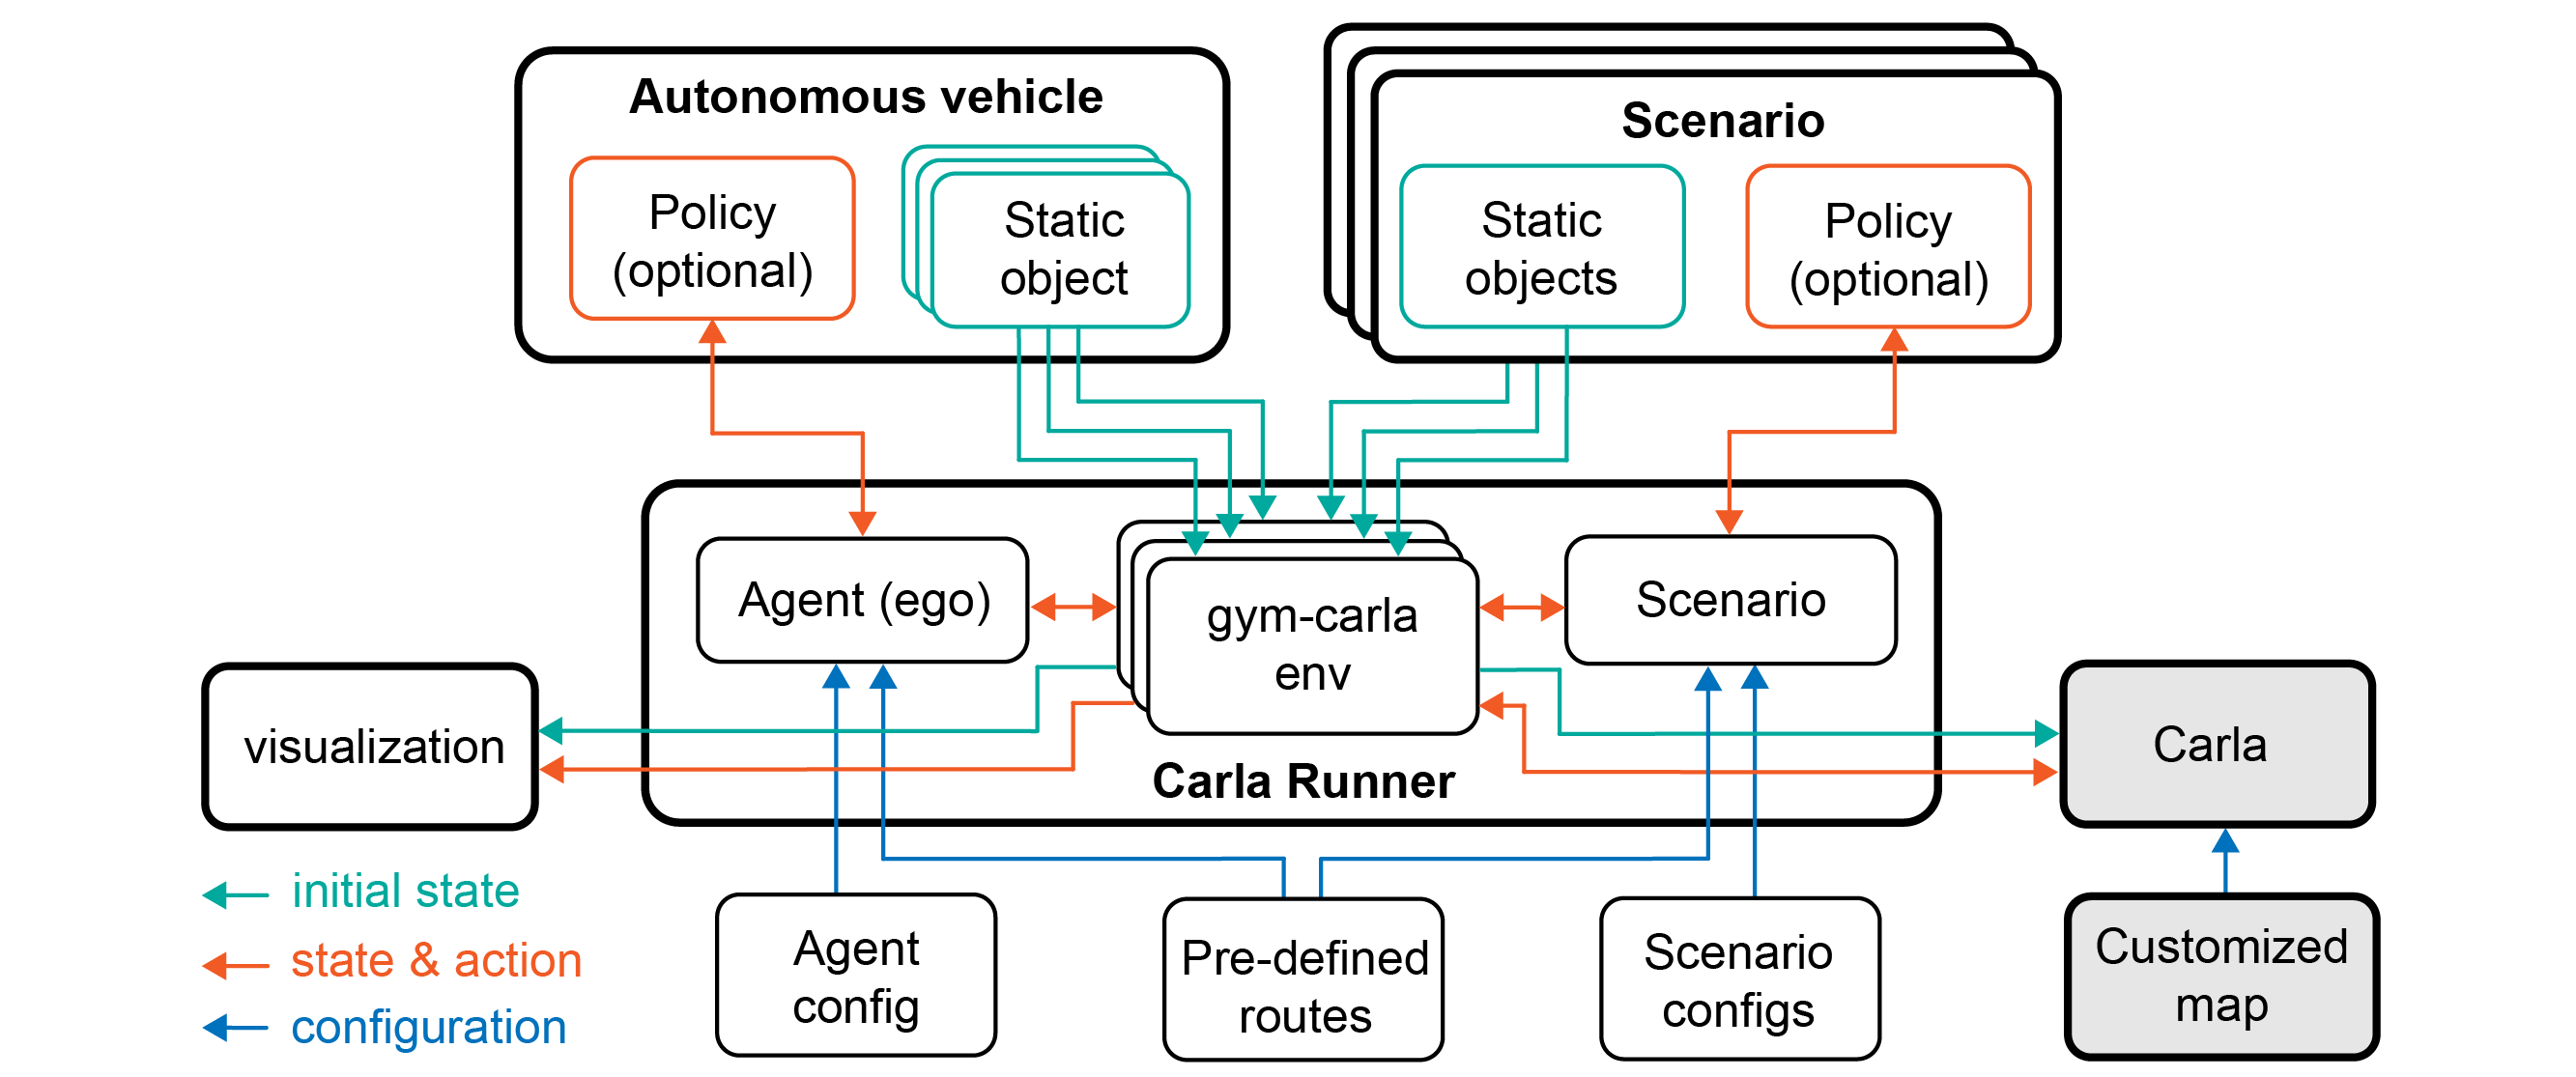
\includegraphics[width=1.0\textwidth]{"images/chatscene项目结构.pdf"}
	\caption{chatscene项目结构}
	\label{fig:chatscene_framework}
\end{figure}
然而,ChatScene 在以下方面存在一定局限:
\begin{itemize}
	\item \textbf{依赖检索}:ChatScene没办法自由生成数据库里不存在的新场景,这种情况限制了它生成创新性场景的能力
	\item \textbf{生成能力有限}:ChatScene没有直接从自然语言生成代码的能力,这导致它处理复杂自然语言描述时有困难
	\item \textbf{多样性受限}:ChatScene的生成结果会受到数据库规模和覆盖范围的制约,这种制约限制了它生成场景的多样性和创新性。
\end{itemize}

为了克服当前存在的这些局限之处,本项目在ChatScene的基础之上开展了创新工作,我们引入了GPT - 4o这类大型语言模型,直接依据自然语言来生成Scenic场景脚本,这种创新方法不但解决了检索方法所存在的局限性,还提升了场景的创新性与多样性水平,通过采用这种方式我们能够生成更为复杂且多样化的场景,为高保真智能驾驶仿真系统构建提供了全新技术路径,此外本项目还通过微调这些大型模型,让其能够更好地适应智能驾驶场景生成的实际需求,从而进一步提高了生成场景的质量和可用性能。